



\documentclass[a4paper,12pt,spanish]{article}

\usepackage[utf8]{inputenc}


\usepackage{blindtext}
%\usepackage{microtype}
\usepackage{amsfonts, amsmath, amsthm, amssymb}
%\usepackage{fancyhdr}
%\usepackage{index}
%\usepackage{multicol}    

%\usepackage{booktabs}

\usepackage[T1]{fontenc}
\usepackage[utf8]{inputenc}
\usepackage{graphicx}
\usepackage[spanish,es-tabla]{babel}
\usepackage{url}
\usepackage{enumitem}

\usepackage[unicode=true, pdfusetitle,
bookmarks=true,bookmarksnumbered=false,bookmarksopen=false,
breaklinks=true,pdfborder={0 0 1},backref=false,colorlinks=false]
{hyperref}

\usepackage{listings}
\usepackage{longtable}


\usepackage{siunitx} %para el sistema internacional
\usepackage[export]{adjustbox}
\usepackage{booktabs} 
\usepackage{subcaption}

\usepackage{float}


\newcommand{\address}[1]{
	\par {\raggedright #1
		\vspace{1.4em}
		\noindent\par}
}

\usepackage[table,xcdraw]{xcolor}


\pagenumbering{gobble}
\include{noNumberPage}
\pagenumbering{arabic}
\setcounter{page}{16}

%tutorial de tablas latex: https://manualdelatex.com/tutoriales/tablas

\usepackage{multirow}

% \usepackage[table,xcdraw]{xcolor}


%Inicio del documento (hasta que se cierre con \end{document}
\begin{document}
	
	
	\title{ Detectores de Centelleo. Absorción de Radiación Gamma}
	
	%\author{Adrián Rivero Fernández}
	\date{}
	
	\maketitle
	
	
	\section{Objetivos de la práctica}
	
	\vspace{\baselineskip}
	
	1. Demostrar la absorción de la radiación gamma por los distintos materiales\\
	
	2. Determinar las curvas de absorción en función del material interpuesto\\
	
	3. Calcular los espesores de semirreducción de materiales para un determinado radionucleido.\\
	
	4. Determinar los coeficientes de absorción lineal y másico.\\
	
	5. Verificar la ley exponencial de absorción.\\
	
	6. Determinar la eficiencia del contador.
	
	
	
	
%	- Fondo
%	- Muestra sin espesor (disminuir fluctuaciones)
	
	
	
	
%	- Representar semilogarítmica espesor-cuentas
%	- Ajustar
	
%	- extrapolar ajuste para 0
%	
%	- Determinar espesor para reducir a mitad las cuentas (semirreducción gráficamente)
%	
	
%	- coeficientes lineal y masico a partir de espesor semirreducción
%	
	
%	- Calcular eficiencia
%	
	
	
	
\begin{figure}[H]
	\centering
	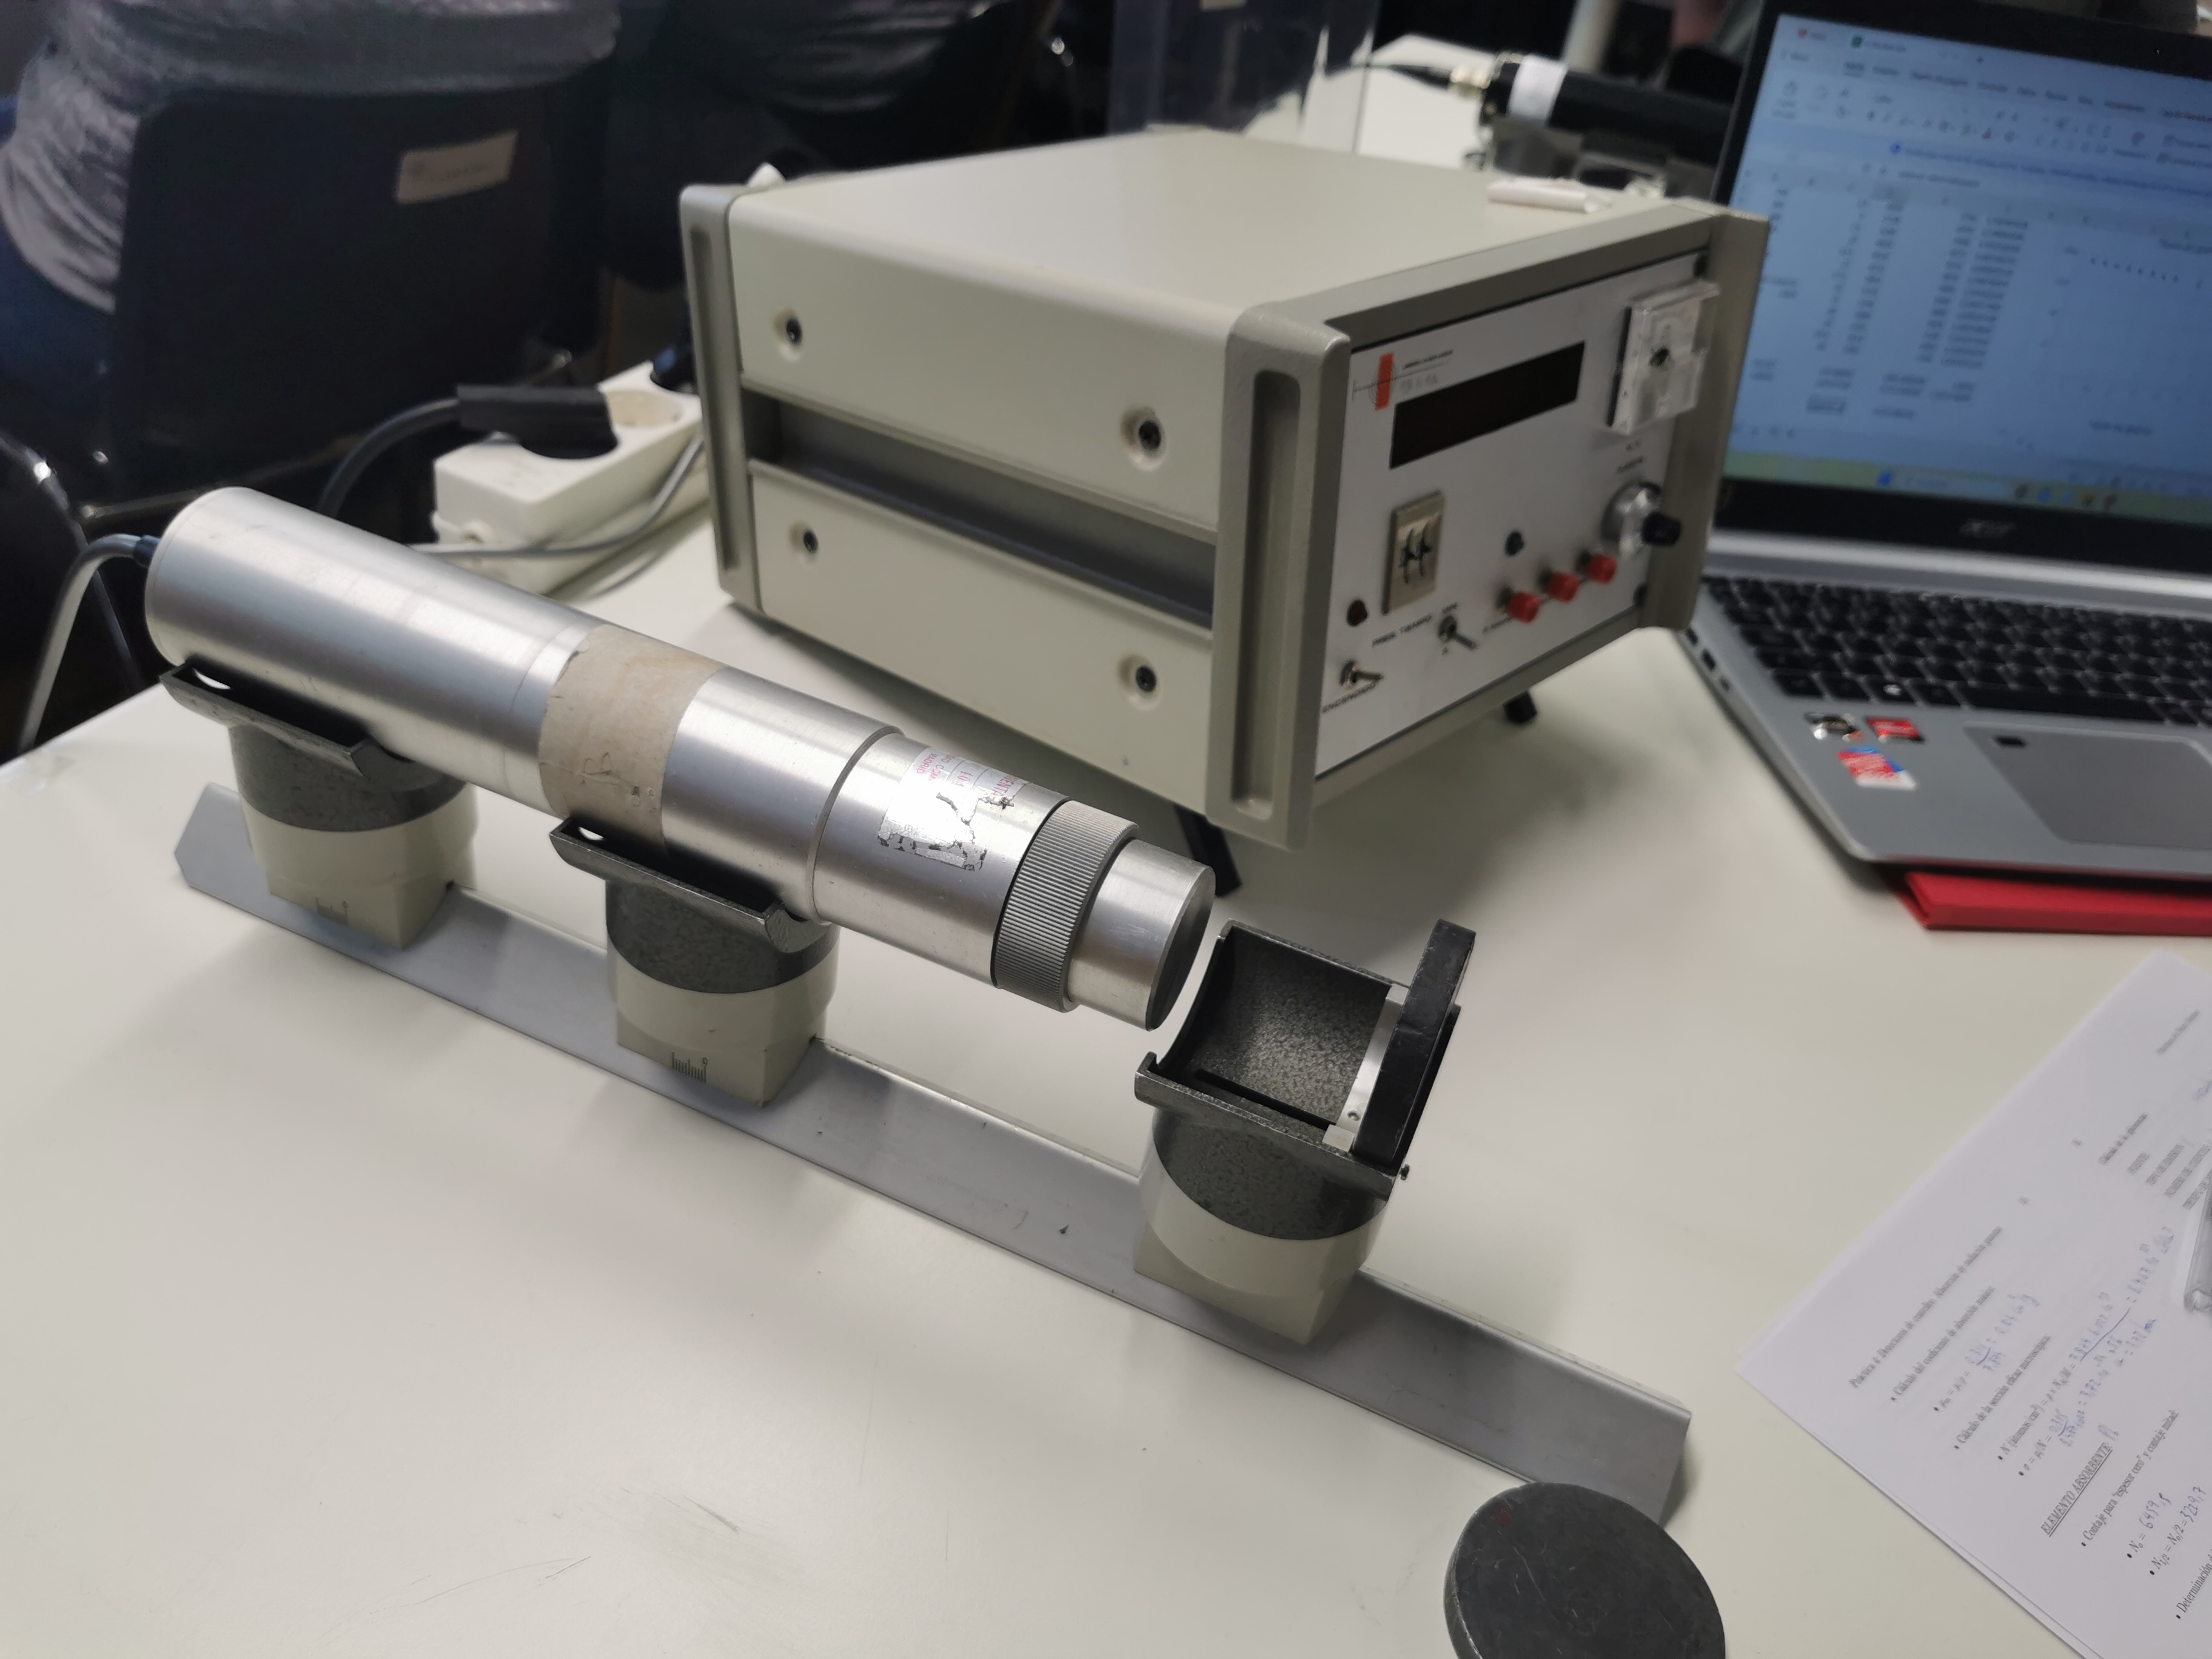
\includegraphics[width=0.7\linewidth]{images/IMG_20240305_121153}
	\caption{Detector de centelleo utilizado}
	\label{fig:img20240305121153}
\end{figure}
	
	
	
	\section{Fondo}
	
	Mediremos la radiación de fondo durante 90s, que luego sustraeremos para el tratamiento de las posteriores medidas de radiación (realizadas con el mismo tiempo).
	
	\begin{table}[H]
		\centering
		\begin{tabular}{c|c|}
			\cline{2-2}
			& Cuentas \\ \hline
			\multicolumn{1}{|c|}{Medida 1 } & 250     \\ \hline
			\multicolumn{1}{|c|}{Medida 2} & 261     \\ \hline
			\multicolumn{1}{|c|}{Medida 3} & 260     \\ \hline
			\multicolumn{1}{|c|}{Medida 4} & 237     \\ \hline\hline
			\multicolumn{1}{|c|}{Media}    & 252     \\ \hline
		\end{tabular}
	\caption{Radiación de fondo para 90s}
	\end{table}

Para reducir las fluctuaciones estadísticas, tomamos una medida sin ningún material entre el emisor y el detector, que nos da:
	
	\[ \text{Medida sin espesor: 6613} 
	\]
	\[ \text{Medida sin espesor menos fondo: } N = 6613 - 252 = 6361
	\]
	

	\section{Aluminio}
	
	%	- Representar semilogarítmica espesor-cuentas
	%	- Ajustar
	
	%	- extrapolar ajuste para 0
	%	
	%	- Determinar espesor para reducir a mitad las cuentas (semirreducción gráficamente)
	%	
	
	%	- coeficientes lineal y masico a partir de espesor semirreducción
	%	
	
	Interponiendo placas de absorbente (en este caso de aluminio), tomamos las medidas de radiación que llega al detector. Los resultados, restando el fondo calculado previamente, están recogidos en la Tabla 2 y representados en la Figura 3
	
	
		
	\begin{figure}[H]
		\centering
		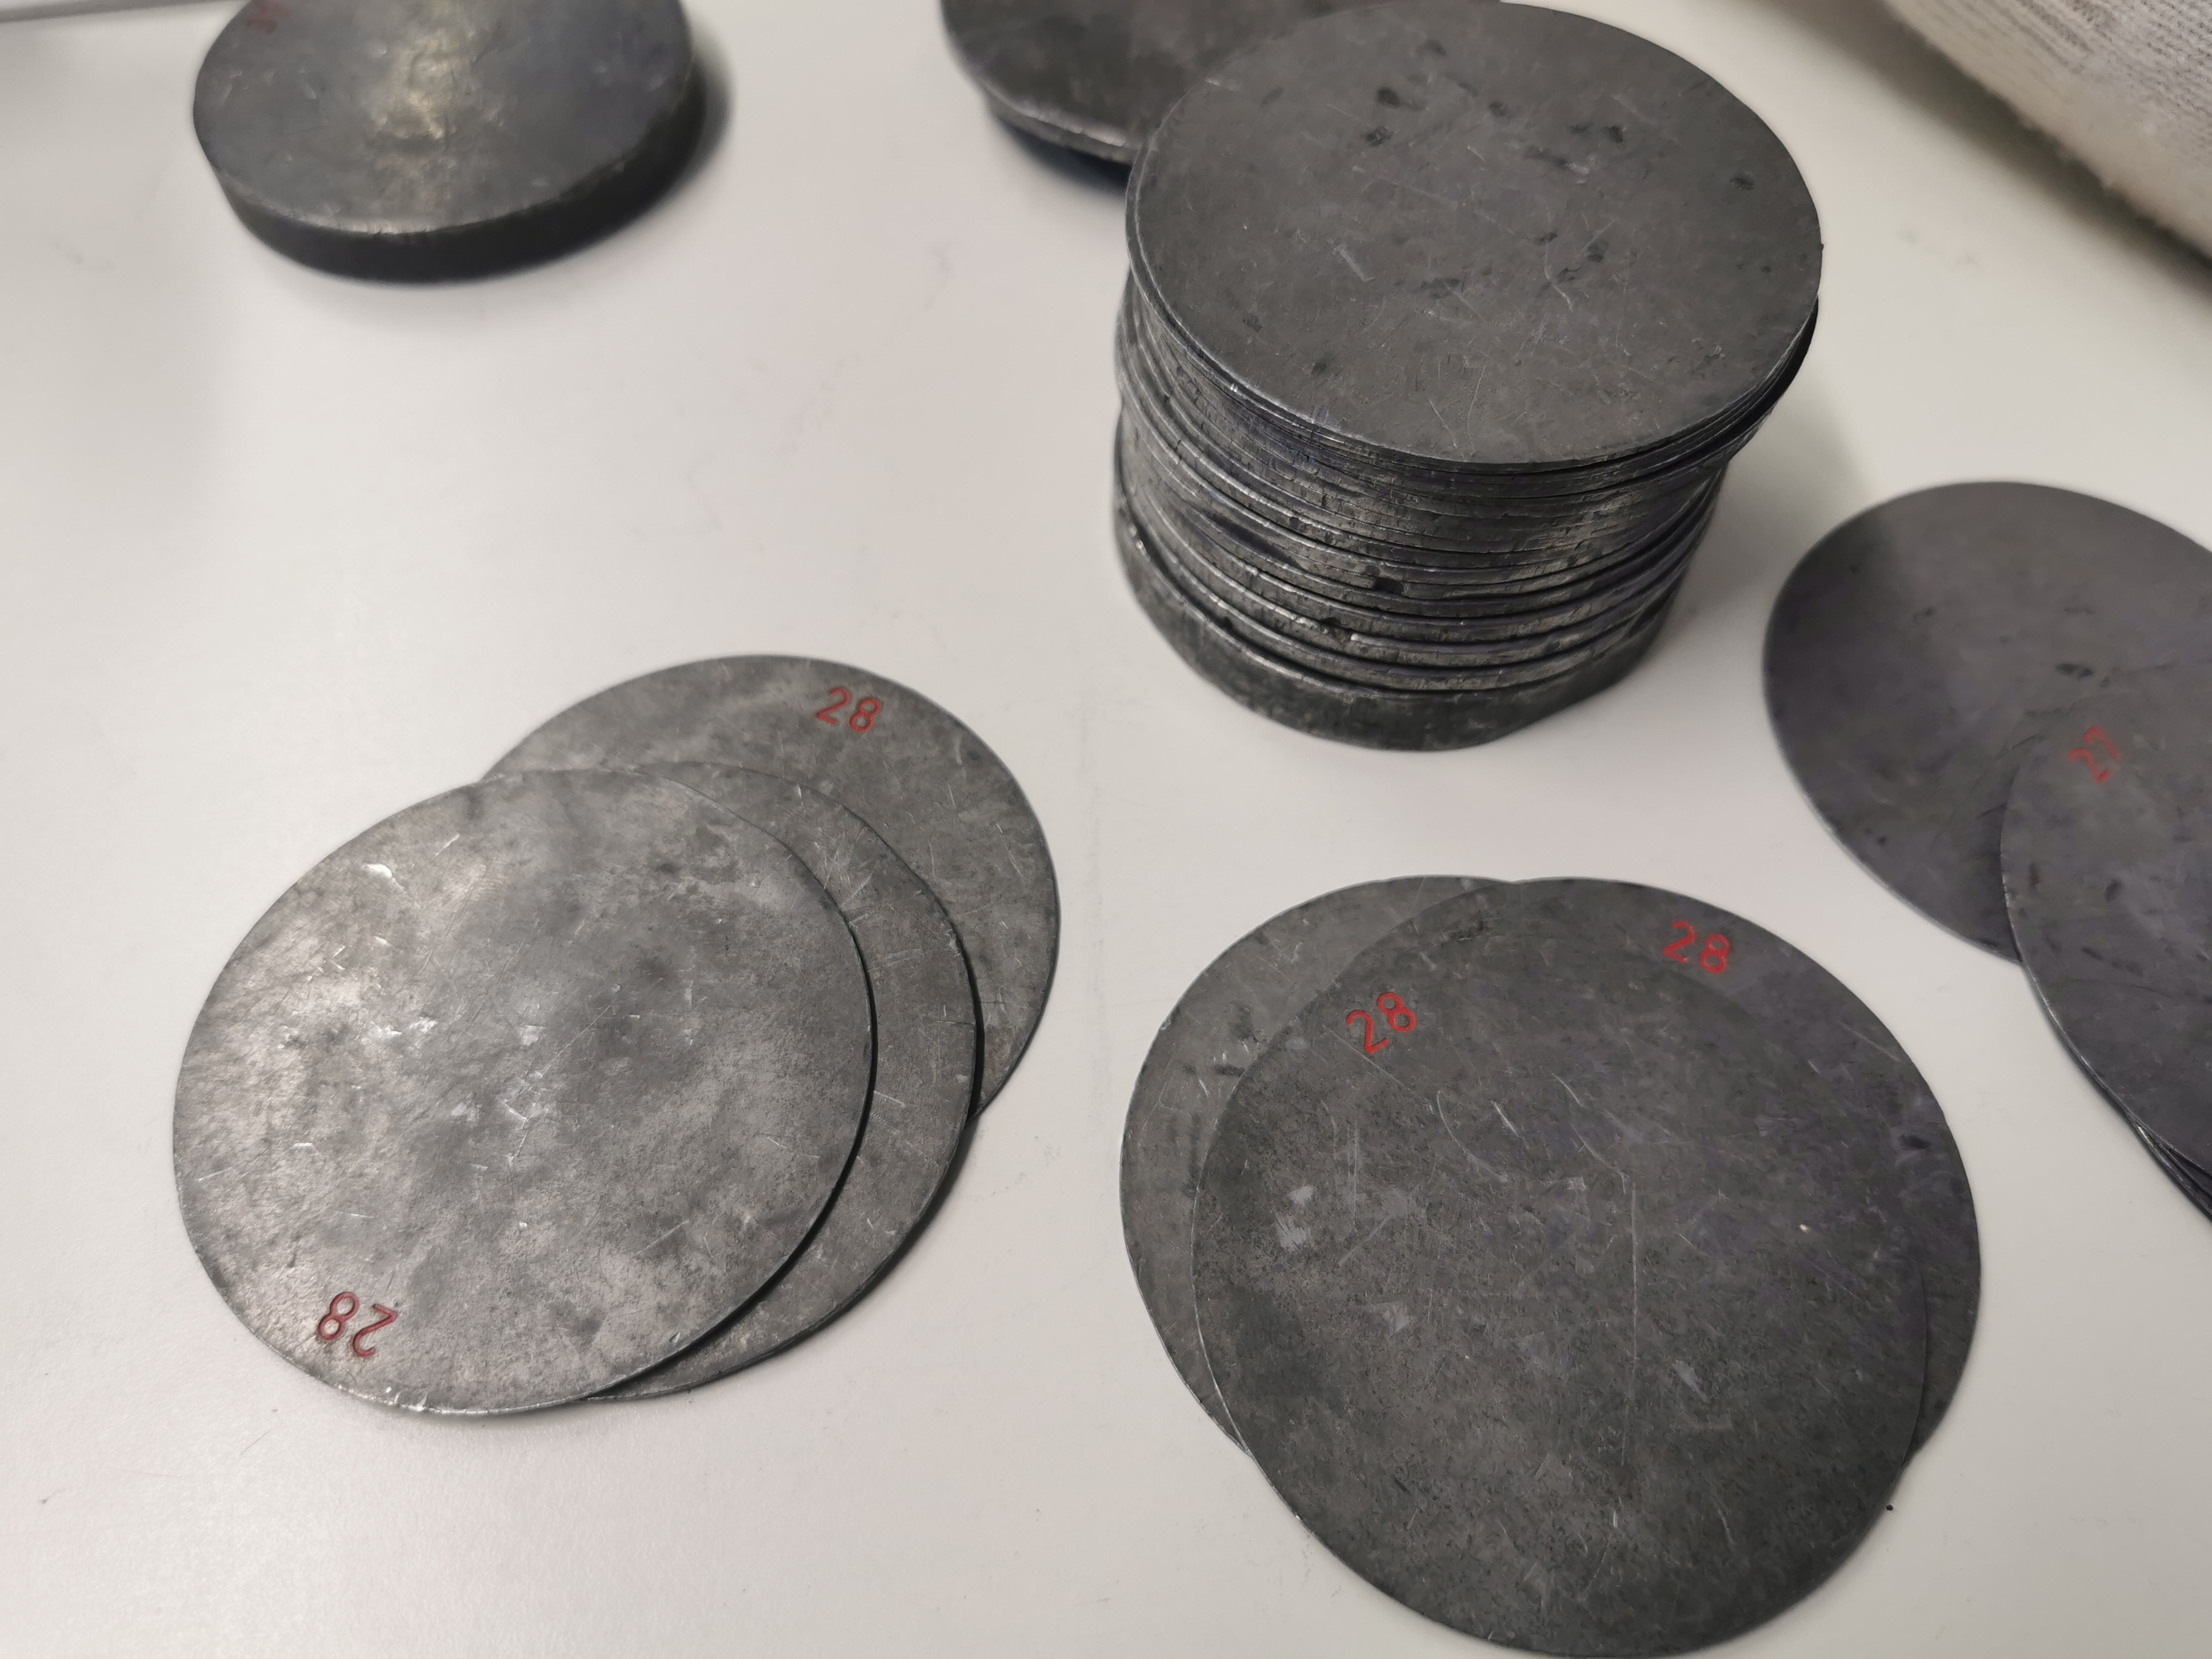
\includegraphics[width=0.7\linewidth]{images/IMG_20240305_121157}
		\caption{Piezas de absorbente (plomo)}
		\label{fig:img20240305121157}
	\end{figure}
	
	
	\begin{table}[H]
		\centering
		\begin{tabular}{|c|c|}
			\hline
			Espesor (mm) & Cuentas \\ \hline
			2,2             & 5809    \\ \hline
			4,4             & 5623    \\ \hline
			6,6             & 5618    \\ \hline
			8,8             & 5492    \\ \hline
			11              & 5455    \\ \hline
			13,2            & 5297    \\ \hline
			15,4            & 4995    \\ \hline
			17,6            & 4882    \\ \hline
			19,8            & 4828    \\ \hline
			24,2            & 4772    \\ \hline
			28,6            & 4358    \\ \hline
			33              & 4230    \\ \hline
			38,3            & 4065    \\ \hline
		\end{tabular}
		\caption{Radiación según espesor de Aluminio}
	\end{table}
	
	
	
	
	
	\begin{figure}[H]
		\centering
		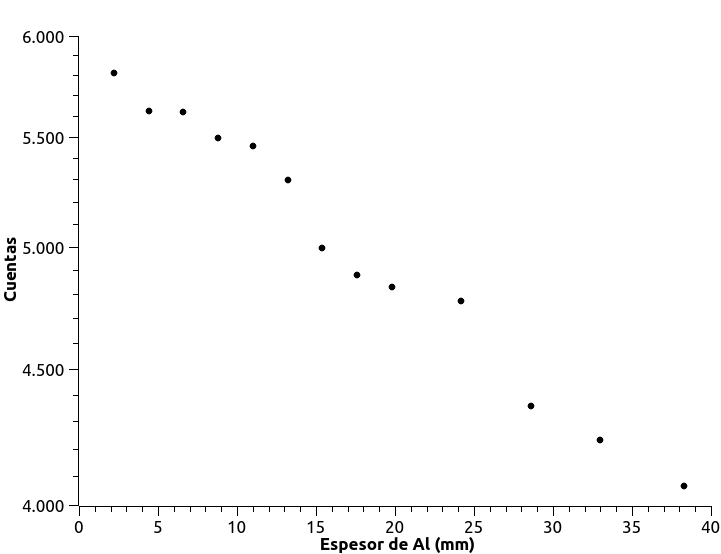
\includegraphics[width=0.9\linewidth]{images/graficas_practica_4/aluminio_cuentas}
		\caption{Radiación según espesor de Aluminio}
		\label{fig:aluminiocuentas}
	\end{figure}
	
	
	La Figura 3, que representa la radiación medida en función del espesor de Aluminio, se ha presentado en escala semilogarítmica, pero su comportamiento exponencial no es tan evidente. Para que la radiación gamma siga la ley exponencial de atenuación, se asume que el material es homogéneo, no hay dispersión ni absorción múltiple y no hay influencias externas significativas. En nuestro caso el sistema puede presentar irregularidades debido a la dispersión en el aire, y la presencia de aire entre nuestras placas de material absorbente. 
	
	
	De los materiales que vamos a utilizar, el Aluminio es el menos denso y, al atenuar peor la radiación, presenta una menor diferencia entre el valor máximo y mínimo medido, lo que hace menos evidente el caracter exponencial de la curva, y lo hace más sensible a imperfecciones y errores.\\
		
	
	Podemos representar el logaritmo de las cuentas frente al espesor para ajustar linealmente a una recta
	
	
		
	\begin{figure}[H]
		\centering
		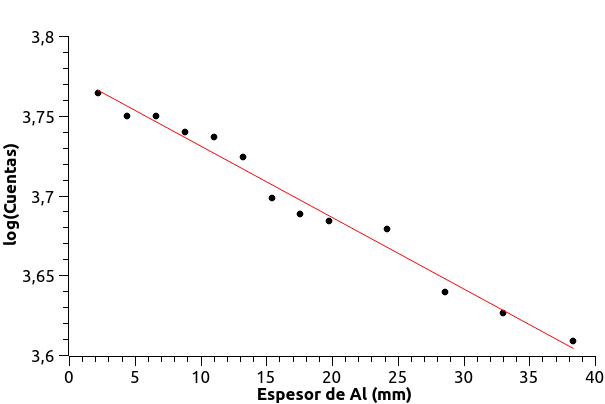
\includegraphics[width=0.7\linewidth]{images/graficas_practica_4/aluminio_ajuste}
		\caption{Ajuste del logaritmo de la radiación frente al espesor para el Aluminio}
		\label{fig:aluminioajuste}
	\end{figure}

	
	\[ log(N) = -0,0045 X + 3,7759
	\]
	\[ N = 10^{-0,0045 X + 3,7759}
	\]
	
	Por tanto, para un espesor nulo,
	\[ X = 0
	\]
	\[N_{0, Al} = 10^{3,7759} = 5968,97\]
	
	
	Este valor de N extrapolado difiere con el valor que medimos previamente en un 6\%, tanto por las causas anteriormente mencionadas como por los errores arrastrados al calcular el logarítmo y realizar la recta de ajuste.
	
	
	El contaje a mitad:
	\[N_{1/2} = N_0 /2 = 2984,49
	\]
	
	Interpolando, obtenemos el espesor de semirreducción:
	\[ X_{1/2} = 66,9 \si{mm}
	\]
	
	El coeficiente de absorción lineal:
	\[ \mu = \frac{\ln 2}{X_{1/2}} = 0,01 \si{mm^{-1}} = 0,1\si{cm^{-1}}
	\]
	
	El coeficiente de absorción másico, teniendo en cuenta que $\rho_{Al} = 2,7 \si{g/cm^3} $:
	\[ \mu_m = \frac{\mu}{\rho} = \frac{0,1\si{cm^{-1}}}{2,7\si{g/cm^3}} = 0,037 \si{cm^2/g}
	\]
	
	Según las figuras del guión, el coeficiente de absorción lineal y másico son, aproximadamente:
	\[ \mu = 0,1\si{cm^{-1}}
	\]
	\[\mu_m = 0,02 \si{cm^2/g}    \]
	
	Dadas las dificultades para comprobarlo con exactitud visualmente, pues se trata de escalas logarítmicas, tienen un parecido bastante razonable con las obtenidas experimentalmente.\\
	
	
	Calculamos la sección eficaz microscópica, teniendo en cuenta $M_{Al}= 27\si{g/mol}$:
	
	\[ N \text{(átomos/cm$^3$)} = \rho \times \frac{N_A}{M} = 0,1 N_A = 6,022\times10^{22}
	\]
	\[ \sigma = \frac{\mu}{N} = \frac{0,1\si{cm^{-1}}}{6,022\times10^{22} \text{(átomos/cm$^3$)}} = 1,66\times 10^{-24} \si{cm^2}
	\]
	

	



	\section{Hierro}
	
	%	- Representar semilogarítmica espesor-cuentas
	%	- Ajustar
	
	%	- extrapolar ajuste para 0
	%	
	%	- Determinar espesor para reducir a mitad las cuentas (semirreducción gráficamente)
	%	
	
	%	- coeficientes lineal y masico a partir de espesor semirreducción
	%	
	
	
	Medimos y representamos de la misma forma para el Hierro, 
	
	
	\begin{table}[H]
		\centering
		\begin{tabular}{|c|c|}
			\hline
			Espesor (mm) & Cuentas \\ \hline
			2,5          & 5793    \\ \hline
			5            & 5476    \\ \hline
			7,5          & 5038    \\ \hline
			10           & 4572    \\ \hline
			12,5         & 4274    \\ \hline
			15           & 3970    \\ \hline
			17,5         & 3600    \\ \hline
			20           & 3464    \\ \hline
			25           & 2888    \\ \hline
			30           & 2428    \\ \hline
			35           & 2159    \\ \hline
			37,5         & 1959    \\ \hline
			39           & 1799    \\ \hline
		\end{tabular}
		\caption{Radiación según espesor de Hierro}
	\end{table}






\begin{figure}[H]
	\centering
	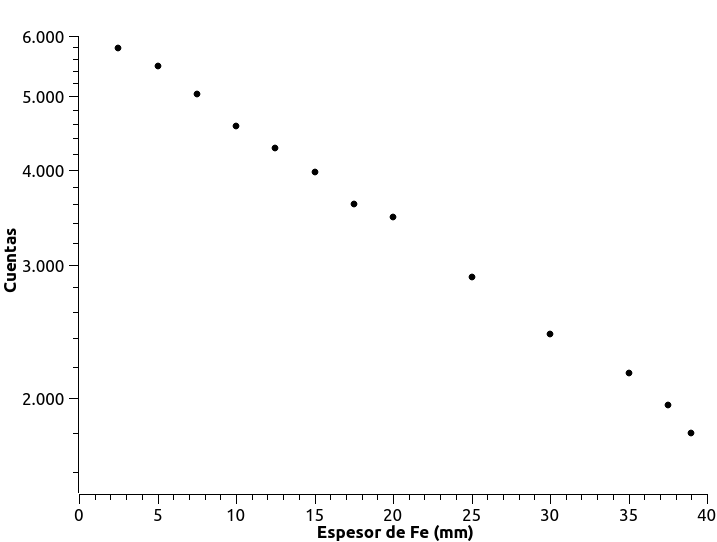
\includegraphics[width=0.9\linewidth]{images/graficas_practica_4/hierro_cuentas}
	\caption{Radiación según espesor de Hierro}
	\label{fig:hierrocuentas}
\end{figure}
	
	Hemos representado en la Figura 5, la radiación medida en función del espesor de Hierro. Para esta gráfica, vemos que se percibe mucho mejor el carácter exponencial que con el Aluminio.\\
	
	Calculamos ahora su expresión:
	
	
	\begin{figure}[H]
		\centering
		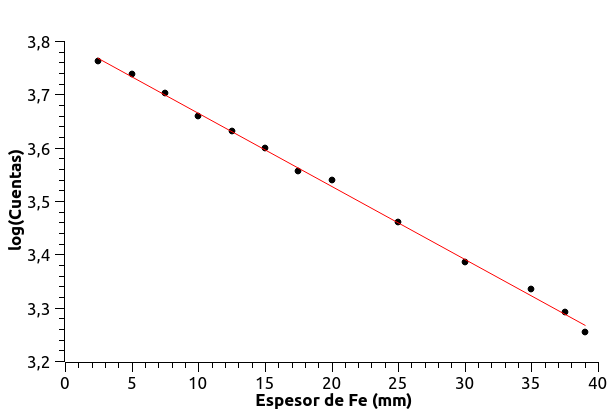
\includegraphics[width=0.7\linewidth]{images/graficas_practica_4/hierro_ajuste}
		\caption{Ajuste del logaritmo de la radiación frente al espesor para el Hierro}
		\label{fig:hierroajuste}
	\end{figure}


	
	\[ log(N) = -0,0137 X + 3,8026
	\]
	\[ N = 10^{-0,0137 X + 3,8026}
	\]
	
	Por tanto, para un espesor nulo,
	\[ X = 0
	\]
	\[N_{0, Fe} = 10^{3,8026} = 6347,46\]

Comparándo este valor extrapolado frente al medido, apenas difieren en un 2\%, que se deberá a los efectos del aire entre placas y errores experimentales. \\


El contaje a mitad:
\[N_{1/2} = N_0 /2 = 3173,73
\]


Interpolando, obtenemos el espesor de semirreducción:
\[ X_{1/2} = 22,0\si{mm}
\]

El coeficiente de absorción lineal:
\[ \mu = \frac{\ln 2}{X_{1/2}} = 0,032 \si{mm^{-1}} = 0,32\si{cm^{-1}}
\]

El coeficiente de absorción másico, teniendo en cuenta que $\rho_{Fe} = 7,87\si{g/cm^3}$:
\[ \mu_m = \frac{\mu}{\rho} = 0,040 \si{cm^2/g}
\]

Calculamos la sección eficaz microscópica, $M_{Fe} = 55,845 \si{g/mol}$:

\[ N \text{(átomos/cm$^3$)} = \rho \times \frac{N_A}{M} = 8,491\times 10^{22} 
\]
\[ \sigma = \frac{\mu}{N} = 3,769\times 10^{-24} \si{cm^2}
\]



	\section{Plomo}
	
	%	- Representar semilogarítmica espesor-cuentas
	%	- Ajustar
	
	%	- extrapolar ajuste para 0
	%	
	%	- Determinar espesor para reducir a mitad las cuentas (semirreducción gráficamente)
	%	
	
	%	- coeficientes lineal y masico a partir de espesor semirreducción
	%	
	
	Realizamos el mismo proceso para absorbentes de Plomo
	
	
	\begin{table}[H]
		\centering
		\begin{tabular}{|c|c|}
			\hline
			Espesor (mm) & Cuentas \\ \hline
			0,9          & 6075    \\ \hline
			1,8          & 5799    \\ \hline
			2,7          & 5586    \\ \hline
			3,6          & 5320    \\ \hline
			4,5          & 5078    \\ \hline
			5,4          & 4786    \\ \hline
			7,2          & 4362    \\ \hline
			9            & 3902    \\ \hline
			10,8         & 3694    \\ \hline
			12,6         & 3146    \\ \hline
			16,2         & 2662    \\ \hline
			19,8         & 2221    \\ \hline
			25,2         & 1707    \\ \hline
			30,6         & 1184    \\ \hline
			36,7         & 849    \\ \hline
		\end{tabular}
		\caption{Radiación según espesor de Plomo}
	\end{table}
	
	
	
	
	
	\begin{figure}[H]
		\centering
		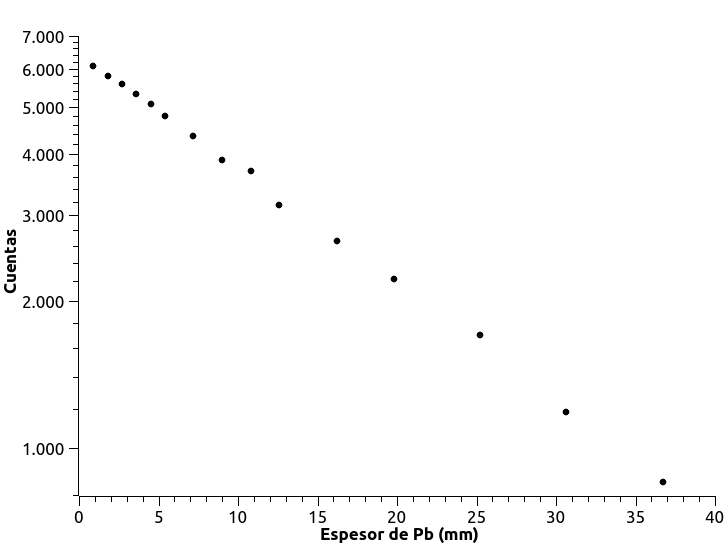
\includegraphics[width=0.9\linewidth]{images/graficas_practica_4/plomo_cuentas}
		\caption{Radiación según espesor de Plomo}
		\label{fig:plomocuentas}
	\end{figure}
	
	
	
	Representadas las cuentas medidas en función del espesor de Plomo en la Figura 7, podemos ver claramente su carácter exponencial. El Plomo es el mejor absorbente de los tres, y el amplio rango de mediciones minimiza la influencia de errores.
	
	\begin{figure}[H]
		\centering
		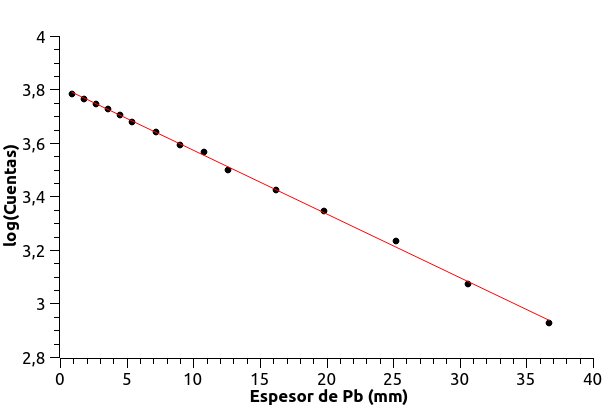
\includegraphics[width=0.7\linewidth]{images/graficas_practica_4/plomo_ajuste}
		\caption{Ajuste del logaritmo de la radiación frente al espesor para el Plomo}
		\label{fig:plomoajuste}
	\end{figure}
	
	
	
	
	
	
	
	
	
	\[ log(N) = -0,0238 X + 3,8102
	\]
	\[ N = 10^{-0,0238 X + 3,8102}
	\]
	
	Por tanto, para un espesor nulo,
	\[ X = 0
	\]
	\[N_{0, Pb} = 10^{3,8102} = 6459,52  \]
	
	En este caso, la diferencia entre el valor extrapolado y el medido es de un 1,5\%, que es la menor de las tres, pero no se aleja demasiado de la del Hierro.
	
	
	
	El contaje a mitad:
	\[N_{1/2} = N_0 /2 = 3229,76
	\]
		
	Interpolando, obtenemos el espesor de semirreducción:
	\[ X_{1/2} = 12,6\si{mm}
	\]
	
	El coeficiente de absorción lineal:
	\[ \mu = \frac{\ln 2}{X_{1/2}} = 0,055\si{mm^{-1}} = 0,55\si{cm^{-1}}
	\]
	
	El coeficiente de absorción másico, teniendo en cuenta $\rho_{Pb} = 11,34\si{g/cm^3}$:
	\[ \mu_m = \frac{\mu}{\rho} = 0,048\si{cm^2/g}
	\]
	
	Las figuras de los guiones también nos proporcionan una estimación de estos dos coeficientes al interpolar en la gráfica, obteniendo unos valores aproximados de
	\[ \mu = 0,6\si{cm^{-1}}
	\]
	\[ \mu_m = 0,03 \si{cm^2/g}
	\]
	De nuevo, se parecen relativamente.\\ 
	
	
	Calculamos la sección eficaz microscópica, con $M_{Pb}= 207,2\si{g/mol}$:
	
	\[ N \text{(átomos/cm$^3$)} = \rho \times \frac{N_A}{M} = 3,296\times 10^{22}
	\]
	\[ \sigma = \frac{\mu}{N} = 16,69\times10^{-24} \si{cm^2}
	\]
	
	
	
	
	
	\section{Eficiencia}
	
	
	La fuente utilizada se trata de una muestra de Sodio-22
	\begin{itemize}
		\item Tipo de emisión: positrones y radiación gamma
		\item Numero de cuentas: $L = 61572$
		\item Actividad inicial: $A_0 = 1\si{\mu Ci}$
		\item Fecha inicial: 28 septiembre 2022
		\item Fecha medida: 5 marzo 2024
		\item Periodo $T_{1/2} = 2,6 \text{ años}$ 
		\item Tiempo de medida: $t = 90\si{s}$
		\item Fondo: $F = 252$
		
		\item Tasa de recuento neta: $A' = (L-F)/t = $
	\end{itemize}
	
	
	La tasa de recuento neta será:
	\[A' = \frac{L-F}{t} = 681,33\si{Bq}\]
	
	La diferencia de tiempo entre el de la actividad inicial y el de la toma de medida es de 1 año y 5 meses, 1,43 años. Por lo tanto la actividad corregida:
	
	\[ A = A_0 \text{e}^{-\lambda t}= A_0 \text{e}^{-\frac{\ln2}{T_{1/2}} t } = 0,684 \si{\mu Ci}
	\]
	\[ A = 0,684 \si{\mu Ci} = 25271 \si{Bq}
	\]
	
	Y por tanto la eficiencia será
	\[ \varepsilon = \frac{A'}{A} = 0,027 \longrightarrow \varepsilon = 2,7 \%
	\]
	
	
	
\end{document}